\chapter{Metodology}
\label{chap:Metodology}

This chapter is about describing the metodology and developments to achieve the project goals. 


\section{Classification}
\label{sec:section_classification}

The classification is a key step in our routine. For being able to be used in multipurpose applications our classification routine must be able to run in real-time. Which means it must be fast and automatic classification.
Our goal is to improve and apply in our routine different approaches of non-visual spraying classification using the current data collected from the system.

\subsection{Statistical Analysis}
In Sjaaks\cite{Sjaaks} work, the author exposed some signal characteristics that can be used to classify the actual spraying mode with a sample of measured current using both time domain and frequency domain analysis.
We acquire the current data frame of 0.5s and through statistical analysis in the signal such as mean value and standard deviation we apply in our automatic classification the relative standard deviation. Which is referred as the sample standard deviation divided by the sample mean values. Figure \ref{fig:sjaaks_statistical_class} illustrate data samples being classified using Sjaaks method.

\begin{figure}[H]
    \centering
    \resizebox{80mm}{!}{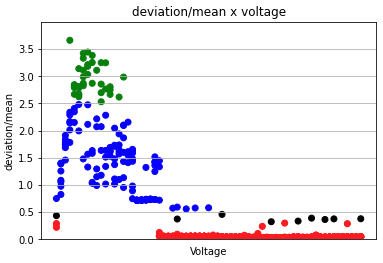
\includegraphics{Figuras/report2/data3_sjaaksgraph2.png}}
    \caption{Sample classification using statistical values. Colors: Green = Dripping; Blue = Intermittent; Red = Cone Jet}
    \label{fig:sjaaks_statistical_class}
\end{figure}

 

This classification by statistical analysis was already implemented in the software library made by the previous student \cite{Monica}.
This method was capable of only classifying dripping, intermittent and cone jet modes. Also in her work, Monica extended the classification to corona or discharge detection.
My contribution was to integrate her work on my control loop model and extend the classification for the multi jet.

To classify the multi jet, after running many steps experiments as shown in figure \ref{fig:raw_data} I noticed that the multi jet signal has a similar shape as the cone jet but with a step in its current mean. 
I also noticed that the cone jet current was almost fixed all its spectrum. 
This effect was cited by Ryan\cite{Ryan}. In his work he defines the relation between current per jet in both cone jet and multi jet modes.

With that, I implemented the classification of the multi jet when the current mean is 1.14 above the expected cone jet current mean. 
The cone jet current can be calculated by the scaling laws\ref{sec:scalling-laws} formula.
The value 1.14 was found by repeating a lot of experiments with the same liquid, but varying the flowrate and the voltage. This means this value is just defined for pure ethanol, the liquid used in all those experiments.
The classification in the algorithm was divided in three steps as shown bellow. The algorithm is shown in \ref{alg:statistical_class}.

        - Sjaak Classification -> Classifies Dripping, Intermittent and Cone Jet
        
        - Monica Classification -> Classifies Corona Sparks

        - João Classification -> Classifies Multi Jet

	The algorithm implemented works in the following way:
	\begin{algorithm}
        \caption{Statistical Classification}\label{alg:statistical_class}
        \begin{algorithmic}
        \Function{statistical\_classification}{$sample$} 

            \State $spray\_mode \gets "Undefined"$;
            \State $mean \gets sample.mean$; 
            \State $std\_deviation \gets sample.std\_deviation$;
            \State $median \gets sample.median$;
            
            \If{ $mean / std\_deviation$ > 2.5}
                \Comment{Sjaak classification \cite{Sjaaks}} 
                \State $spray\_mode \gets "Dripping"$;
            \ElsIf{$ 2.5 < mean / std\_deviation < 2.5 \And mean / std\_deviation > 0.3 $}
                \State $spray\_ mode \gets "Intermittent"$;
            \ElsIf{ $mean / std\_deviation$ < 0.3}
                \State $spray\_ mode \gets "Cone Jet"$;
                \State $cone\_jet\_mean \gets mean$;
            \EndIf

            \If{ $mean / std\_deviation$ > 2.5}
                \Comment{Monica classification \cite{Monica}} 
            \EndIf

            \If{ $spray\_mode == "Cone Jet"$}
                \Comment{João classification} 
                \If{ $cone\_jet\_mean > 1.14 \times mean$}
                    \State $spray\_ mode \gets "Multi Jet"$;
                \EndIf
            \EndIf

            \Return $spray\_ mode$;
        \EndFunction
        \end{algorithmic}
    \end{algorithm}



\section{Routine Sequences}
\label{sec:routine_sequences}

    The program developed is capable of running different types of routines. The code is also easy to implement new routines.
    Continuing the methodology, in the setup json file there is a "sequence" attribute which can be chosen between "ramp", "step", "map" or "control".
    The controller thread will manage what the algorithm must do for each sequence.
    Following our control model\ref{fig:control_model_fig}, the controller outputs are the actuators signal.
    The sampling rate is fixed to 0.5 seconds for all the experiments, and it's managed by the data\_acquisiton thread\ref{subsec:data_aquisition}.


\subsection{Ramp}



\subsection{Step}
\label{subsec:step_routine}


\begin{algorithm}
    \caption{STEP sequence in controller thread}\label{alg:stepping_algorithm}
    \begin{algorithmic}
    \Procedure{STEP}{$voltage\_start,voltage\_stop$} 
        \State $voltage \gets voltage\_start$
        \While{$voltage \leq voltage\_stop$} \Comment{scanning voltage range}
            \State \Call{send\_voltage\_command}{voltage}
            \State \Call{sleep}{step \_time}
            \State $voltage \gets voltage + step\_size$
        \EndWhile
    \EndProcedure

    \end{algorithmic}
\end{algorithm}

\subsection{Map}

The map that will be explained bellow is the most relevant sequence in this work. This type of experiment saves human work and time, create a precise analysis and can be compared with previous works for validation of methodology.
The purpose is to map the operational window, seen in Figure \ref{fig:ganan_calvo_fig}, that can be defined where the cone jet spraying mode can be stabilized based on the flow rate, voltage and the setup configuration\cite{gananCalvo}.

    \begin{figure}[H]
        \center
        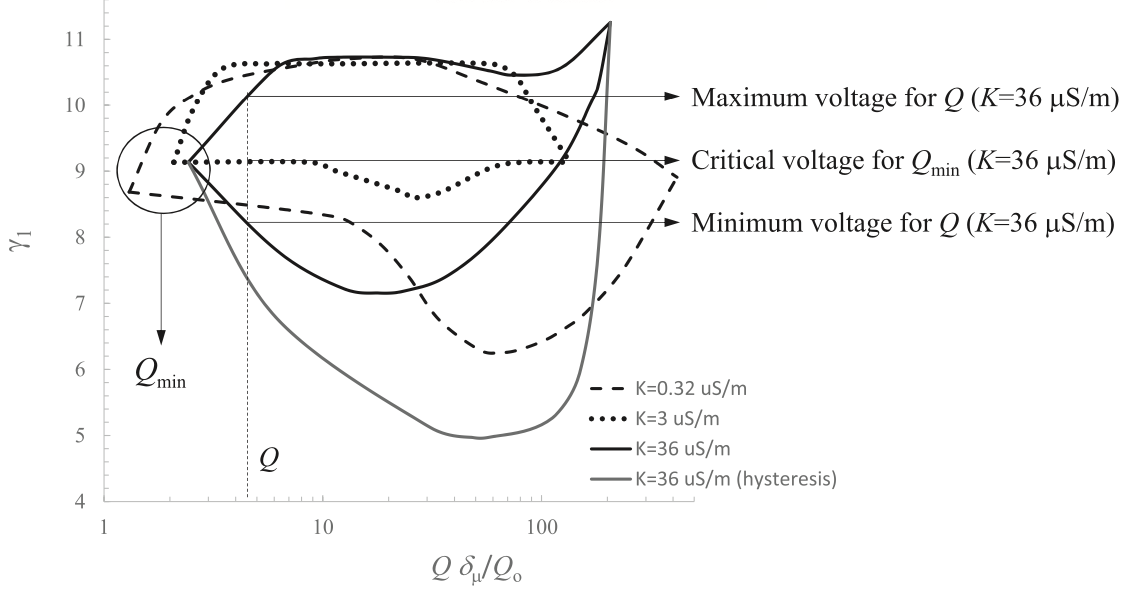
\includegraphics[width=13cm]{Figuras/ganan_calvo_map.png}
        \caption{Domains of existence (stability) of Taylor Cone Jets. \cite{gananCalvo} . The window formed by these points is where the system operated in the stable cone-jet. Operational windows depend of the liquid and configuration setup. Different windows are represented for different liquid conductivity. The X and Y axis are non-dimensional representation of electric potential and liquid flow rate, respectively.}
        \label{fig:ganan_calvo_fig}
    \end{figure}

To reach certain map it is necessary to traverse flow rate and voltage values acquiring samples.
The flow rate (X axis) and voltage (Y axis) values for each experiment can be configured in the setup.json file.
The algorithm for this sequence is a copy of the step sequence\ref{subsec:step_routine} for each flow rate chosen. It is illustrated in the algorithm \ref{alg:mapping_algorithm}.


    \begin{algorithm}
        \caption{MAP sequence in controller thread}\label{alg:mapping_algorithm}
        \begin{algorithmic}
        \Procedure{MAP}{$flowrate\_values$} 
            \ForAll{flowrate\_values}  \Comment{scanning in the flowrate range}
                \State \Call{send\_flowrate\_command}{flowrate}
                \State $voltage \gets voltage\_start$
                \While{$voltage \leq voltage\_stop$} \Comment{scanning in the voltage range}
                    \State \Call{send\_voltage\_command}{voltage}
                    \State \Call{sleep}{step \_time}
                    \State $voltage \gets voltage + step\_size$
                \EndWhile
            \EndFor
        \EndProcedure

        \end{algorithmic}
    \end{algorithm}

    In Figure \ref{fig:map2Data_fig} we can see the data acquired in this mapping experiments. The liquid used is pure ethanol. 
    Note that the experiment is composed of loops that increase voltage, change flowrate and repeat.


    \begin{figure}[H]
        \center
        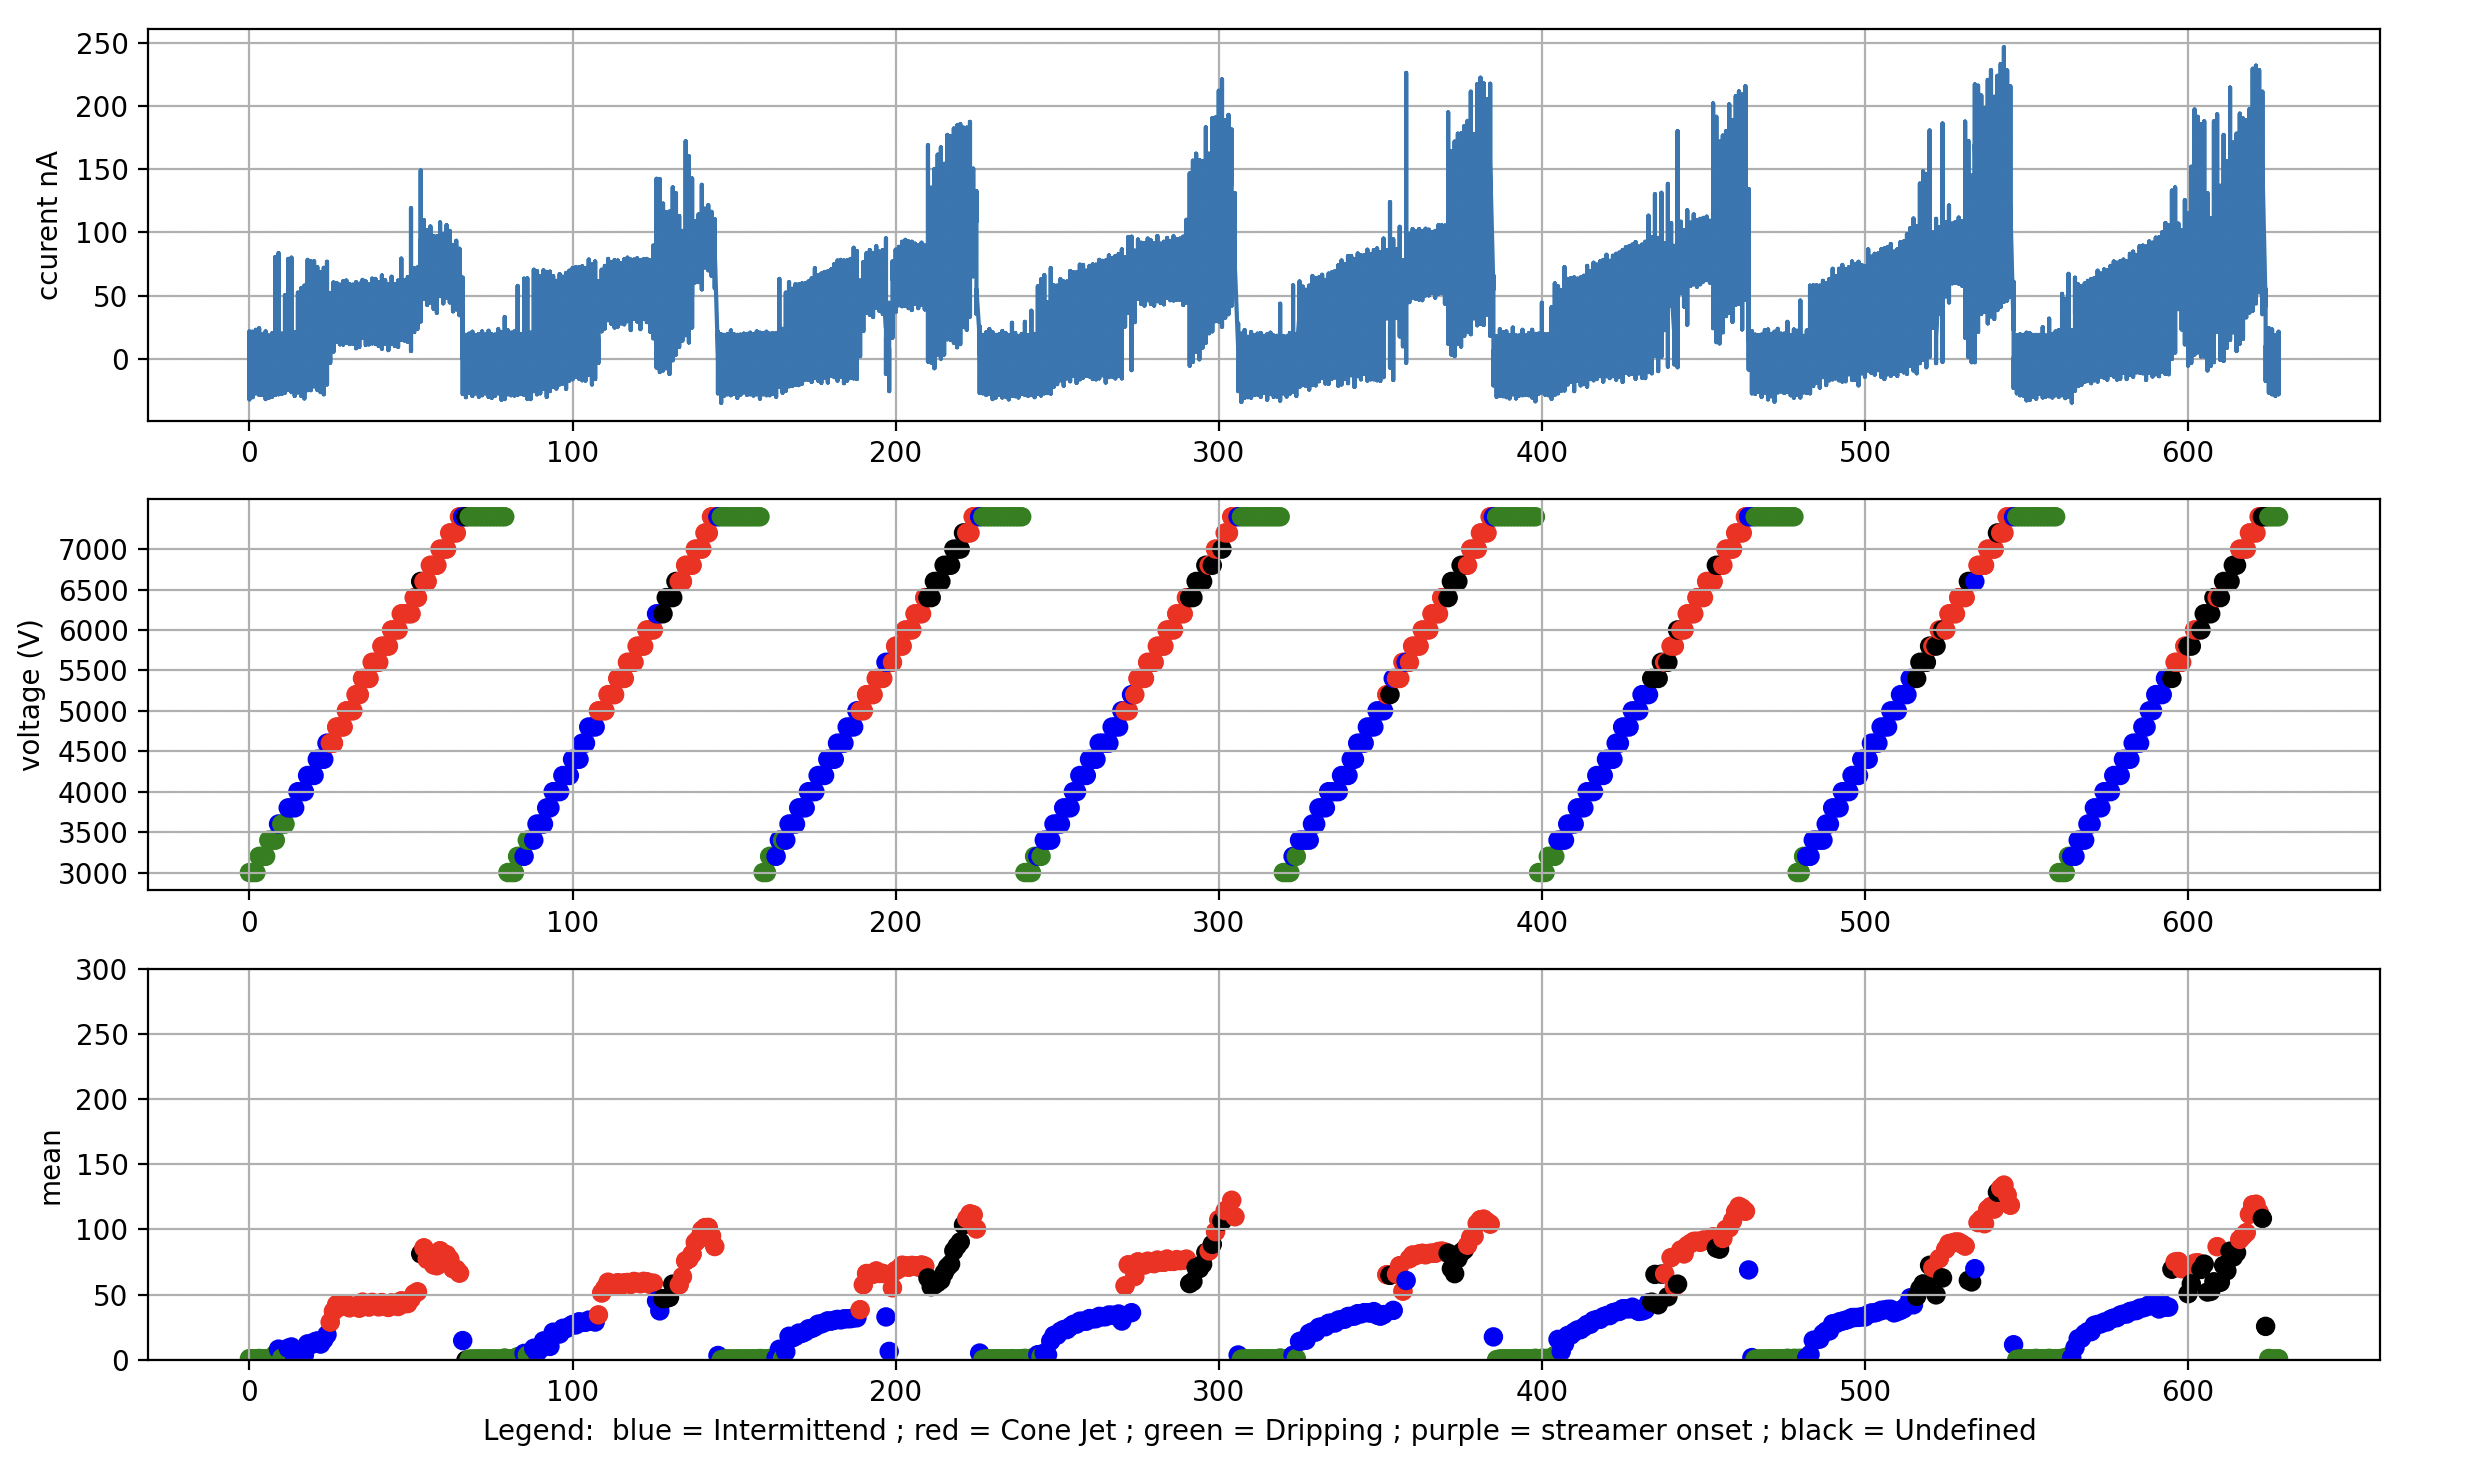
\includegraphics[width=15cm]{Figuras/report2/map2Data.png}
        \caption{Mapping Experiment data collected. The figure has 3 graphs with shared x axis representing the samples collected. The first is the current values collected through all the experiment.
        The second is the voltage values applied in each window of data collected. The colors represent the spraying classification defined by our routine.
        The third graph shows the current mean value of each data sample.}
        \label{fig:map2Data_fig}
    \end{figure}

    With all the data collected, classified and saved in real time, we can do further analysis and studies. For example, Figure \ref{fig:map3Data_fig} illustrate the data classified by our algorithm and displayed in a Voltage X FlowRate range of spraying modes with a specific liquid setup so that we can compare the automatic results with previous researchs, such as showed in figure \ref{fig:ganan_calvo_fig} and validate the algorithm.

    \begin{figure}[H]
        \center
        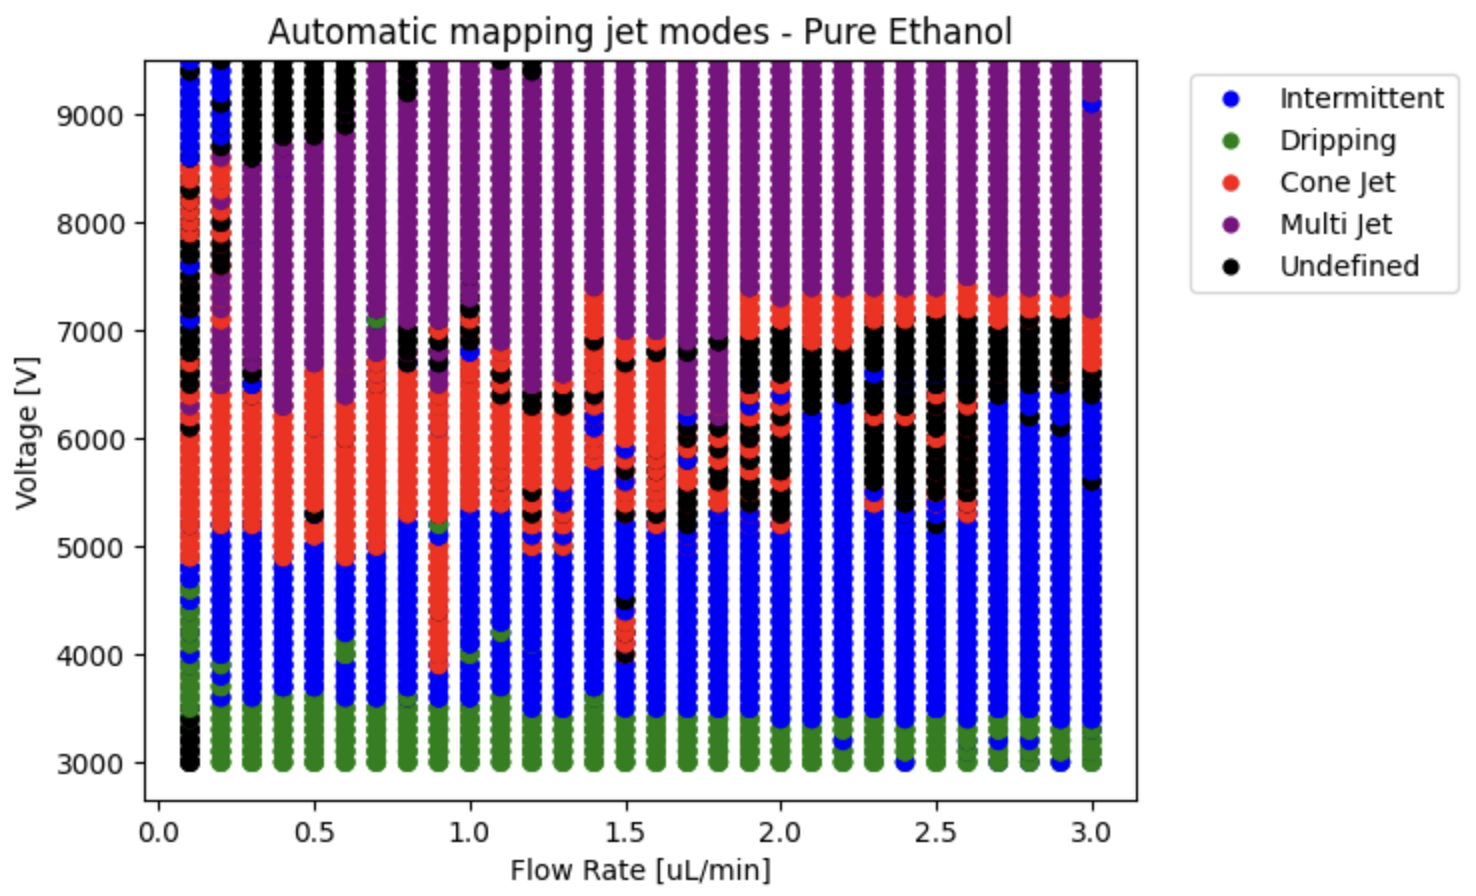
\includegraphics[width=15cm]{Figuras/report4/map-2023-03-02.png}
        \caption{Mapping Experiment for pure ethanol in ambient conditions with our capillary setup. The map shows the stability region of each electrospraying mode in the voltage and flowrate range.}
        \label{fig:map3Data_fig}
    \end{figure}



\subsection{Control}

    The control sequence is the only from our list of sequences that actually uses the feedback value. 
    As it is a closed loop control system the controller must be able to stabilize the system in the desired conditions.






\clearpage